\documentclass[12pt,oneside]{article}
%\usepackage[a4paper, left=2.5cm, right=2.5cm, top=2.5cm, bottom=1in]{geometry}
\usepackage[a4paper]{geometry}

\usepackage{amsmath}
\usepackage{amssymb}
\usepackage{amstext}
\usepackage{amsthm}

% for bibliography:
%\usepackage{comment}
%\usepackage[ backend=biber, style=chicago ]{biblatex}
%\usepackage[
%backend=biber,
%style=numeric,
%]{biblatex}
%\DeclareNameAlias{default}{last-first}

%\addbibresource{biblio.bib}
% see:
% https://www.sharelatex.com/learn/Bibliography_management_in_LaTeX#The_bibliography_file

\usepackage[export]{adjustbox}
\usepackage{tikz}
\usetikzlibrary{arrows}
\usetikzlibrary{scopes}
\usetikzlibrary{babel}

% For cross references
%\usepackage{hyperref}
\usepackage[colorlinks = true]{hyperref}
\usepackage[catalan]{varioref}
%\usepackage{cleveref}
%hyperref configuration so that it doesn't contrast so much colorlinks,
\usepackage{xcolor}
\hypersetup{
   linkcolor={black},
   citecolor={black},
   %linkcolor={red!50!black},
   %citecolor={blue!50!black},
   urlcolor={blue!80!black} }

% Custom Math operators (functions not in italic in math mode):
\DeclareMathOperator{\arcsec}{arcsec}
\DeclareMathOperator{\arccot}{arccot}
\DeclareMathOperator{\arccsc}{arccsc}
\DeclareMathOperator{\cis}{cis}

\usepackage[spanish]{babel} %Names in spanish
\usepackage[utf8]{inputenc} %Use unicode
\usepackage[T1]{fontenc}
\usepackage{csquotes} %For bibliography quotations
%\DeclareQuoteAlias{spanish}{catalan}

\usepackage{array}
\usepackage{float}  %Force tables and images position (H and H!)
\usepackage{wrapfig} %Wrap images like in HTML
\usepackage{listings} %For code blocks
\usepackage{color}  %Custom colors for syntax highlight in listings

\usepackage{tabularx,colortbl, booktabs} %Better tables
\usepackage[alsoload=hep]{siunitx} %Better tables and SI units and uncertainties
\usepackage{longtable}
\sisetup{separate-uncertainty=true}
\sisetup{locale = FR} %commas and so on for spanish
\sisetup{
  per-mode=fraction,
  fraction-function=\nicefrac
}
\usepackage{multirow}
\usepackage{multicol}
\usepackage{makecell}%Slit cell in lines and more formating options inside table

\usepackage{datetime} %To customize date

\newdateformat{monthyeardate}{%
    \monthname[\THEMONTH], \THEYEAR}
%Now \monthyeardate\today gives the date without the day

\usepackage[framemethod=tikz]{mdframed}
\usepackage{nicefrac} %nice fractions in one line

%Subfigures
\usepackage{subcaption}
\usepackage{relsize} %Bigger math with mathlarger{___}

\usepackage[bottom]{footmisc} %footnote at the bottom

%\usepackage{multicol}

%\definecolor{codegreen}{rgb}{0,0.6,0} 
%\definecolor{codegray}{rgb}{0.5,0.5,0.5}
%\definecolor{codepurple}{rgb}{0.58,0,0.82}
%\definecolor{backcolour}{rgb}{0.95,0.95,0.92}

%\lstdefinestyle{mystyle}{ backgroundcolor=\color{backcolour},
    %commentstyle=\color{codegreen}, keywordstyle=\color{blue},
    %numberstyle=\tiny\color{codegray}, stringstyle=\color{red},
    %identifierstyle=\color{black}, basicstyle=\footnotesize,
    %%breakatwhitespace=false,         
    %breaklines=true,                 
    %%captionpos=b,                    keepspaces=true,                 
    %numbers=left,                    numbersep=5pt,
    %showspaces=false,                
    %%showstringspaces=false, showtabs=false,                  
    %tabsize=4 }

%\lstset{style=mystyle}


%%\renewcommand{\figurename}{Fig.} \renewcommand{\tablename}{Tabla}
%%tabla-es in babel better

%\definecolor{lightblue}{RGB}{135,206,250}

%% Add command before appendix session for page numbering: A-1
%\newcommand{\appendixpagenumbering}{
    %\break
    %\pagenumbering{arabic}
    %\renewcommand{\thepage}{\thesection-\arabic{page}}
%}

%\newcommand{\whitepage}{
    %\clearpage\thispagestyle{empty}\addtocounter{page}{-1} \newpage \clearpage
%}



%\geometry{margin=1in}

\title{
   Probabilidad y estadística - B7 \\
   \large 
   - Estudio del oleaje y el viento en Nazaré y Jaws -
}
\author{
  Aleix Boné \and
  Alex Herrero \and
  Albert Mercadé
}
\date{
  \today
}

\begin{document}
\maketitle
%\tableofcontents

\begin{abstract}
% resumen
% <= 250 palabras
\end{abstract}

\section{Introducción}%
\label{sec:introduccion}
% Justificación + objetivos
Dentro del ámbito del surf hay muchos factores a tener en cuenta en cuanto  a lo que se refiere a la ``ola perfecta''. Entre ellos, dos de los más importantes son el tamaño de la ola y la velocidad del viento.

En este caso queremos comparar dos de los surf spots\footnote{Lugar con olas surfeables} con las olas más grandes del mundo a lo largo de la historia; Nazaré en Portugal y Jaws en Peahi, Hawaii. Paralelamente observaremos qué relación tiene la velocidad de viento con el tamaño de las olas en ambos sitios.

\section{Recogida de datos}%
\label{sec:recogida_de_datos}

Para realizar nuestro análisis recogimos datos de viento y altura de olas de
dos localizaciones distintas. Escogimos dos playas conocidas por sus buenas
olas para hacer surf: Nazaré, Portugal y Jaws, Hawaii.

Pudimos obtener datos de oleaje y viento del archivo de \emph{WindGuru}
\footnote{\url{https://www.windguru.cz/archive.php}}. Con un script de
Python\footnote{El código se puede ver en el anexo
  \ref{sec:codigo_extraccion_de_datos}} extrajimos datos de la altura de las
olas y viento en periodos de 3 horas de 2006 hasta hoy. En el caso de Nazaré
obtuvimos datos de 4377 días (35016 periodos de 3 horas) y en Jaws 3338 días
(26704 periodos de 3 horas).

\section{Métodos}%
\label{sec:metodos}
% Métodos (unidades, variables, análisis)

\section{Resultados}%
\label{sec:resultados}
% Descriptiva más inferencia



\begin{figure}[!ht]
\label{fig:wind_waves_jaws}
  \caption{Velocidad de viento vs. Altura de olas en Jaws, Hawaii}
\centering
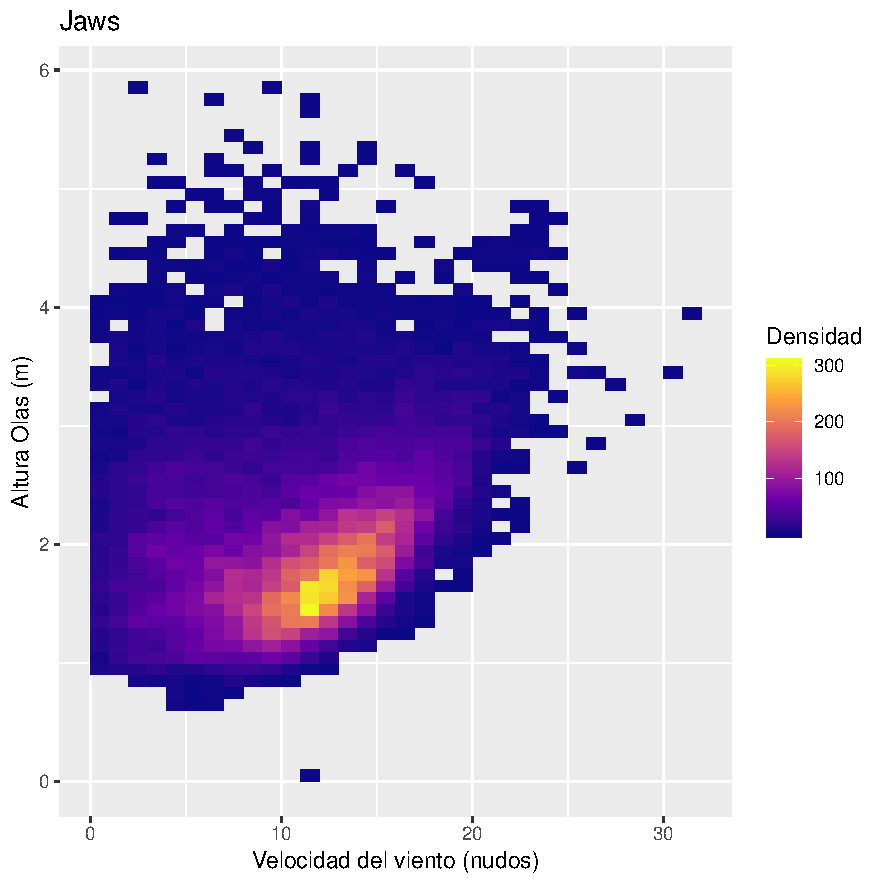
\includegraphics[width=0.6\textwidth]{./figures/jaws.pdf}
\end{figure}

\begin{figure}[!ht]
\label{fig:wind_waves_nazare}
  \caption{Velocidad de viento vs. Altura de olas en Nazaré, Portugal}
\centering
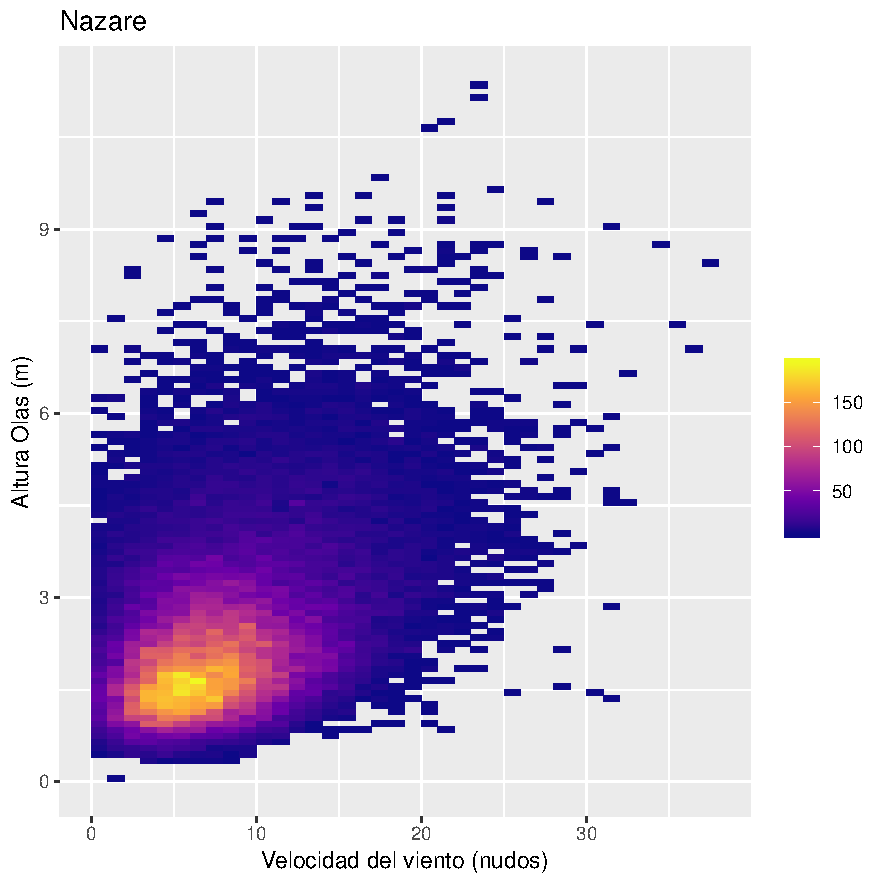
\includegraphics[width=0.6\textwidth]{./figures/nazare.pdf}
\end{figure}



\section{Discusión}%
\label{sec:discusión}


\pagebreak
\appendix

\section{Código extracción de datos}%
\label{sec:codigo_extraccion_de_datos}

\lstinputlisting[language=Python]{./process.py}

\end{document}

% vim:sw=2:ts=2:et:spell:spelllang=es:
